%-----------------------------------------
\begin{frame}
\frametitle{Immediate hybrid - direct aggregation}
    \begin{figure}      
    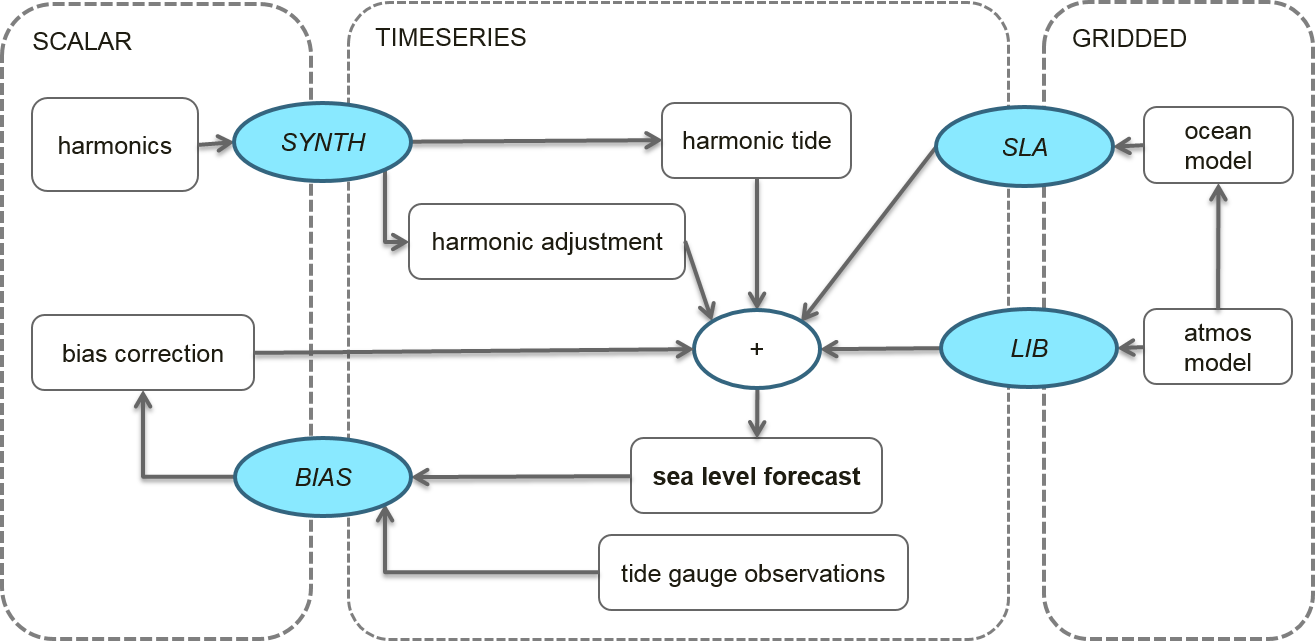
\includegraphics[width=\textwidth]{figures/diagrams/aggSL_schematic_abstract.png}
    \end{figure}
\end{frame}
%-----------------------------------------
\begin{frame}
\frametitle{Immediate hybrid}
    \begin{figure}      
    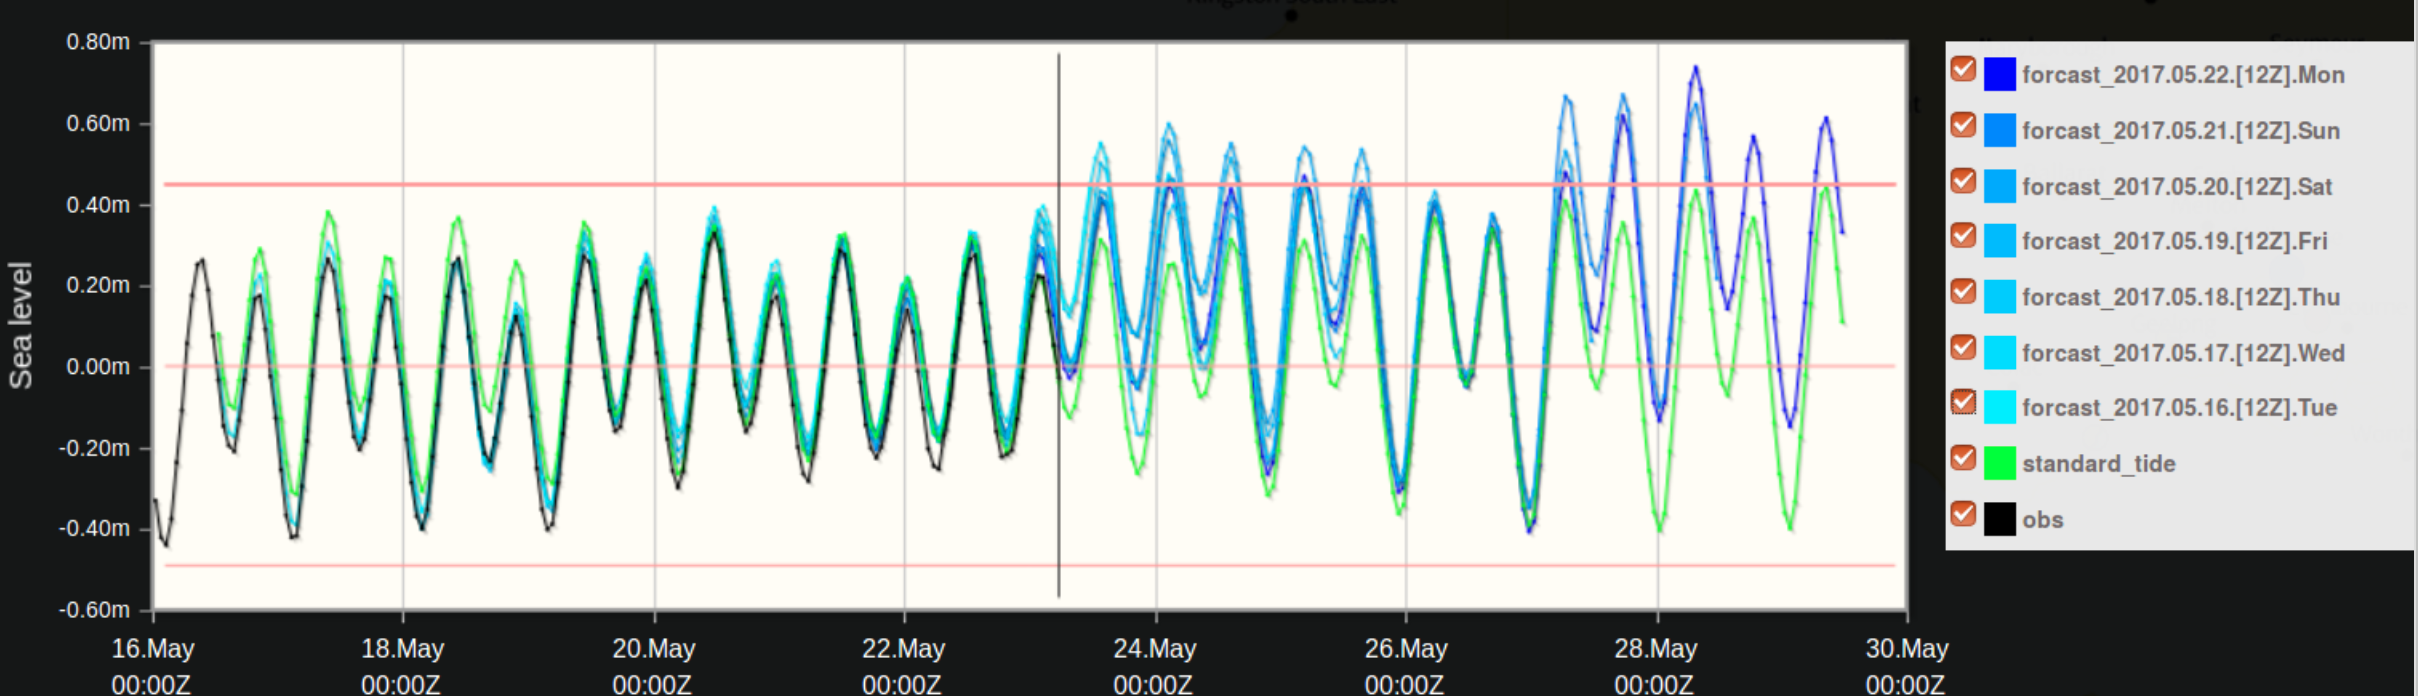
\includegraphics[width=\textwidth]{figures/plots/forecast_eg.png}
    \end{figure}
\end{frame}
%-----------------------------------------
\begin{frame}
\frametitle{Spatial discretisation of the coast}
    \begin{figure}      
    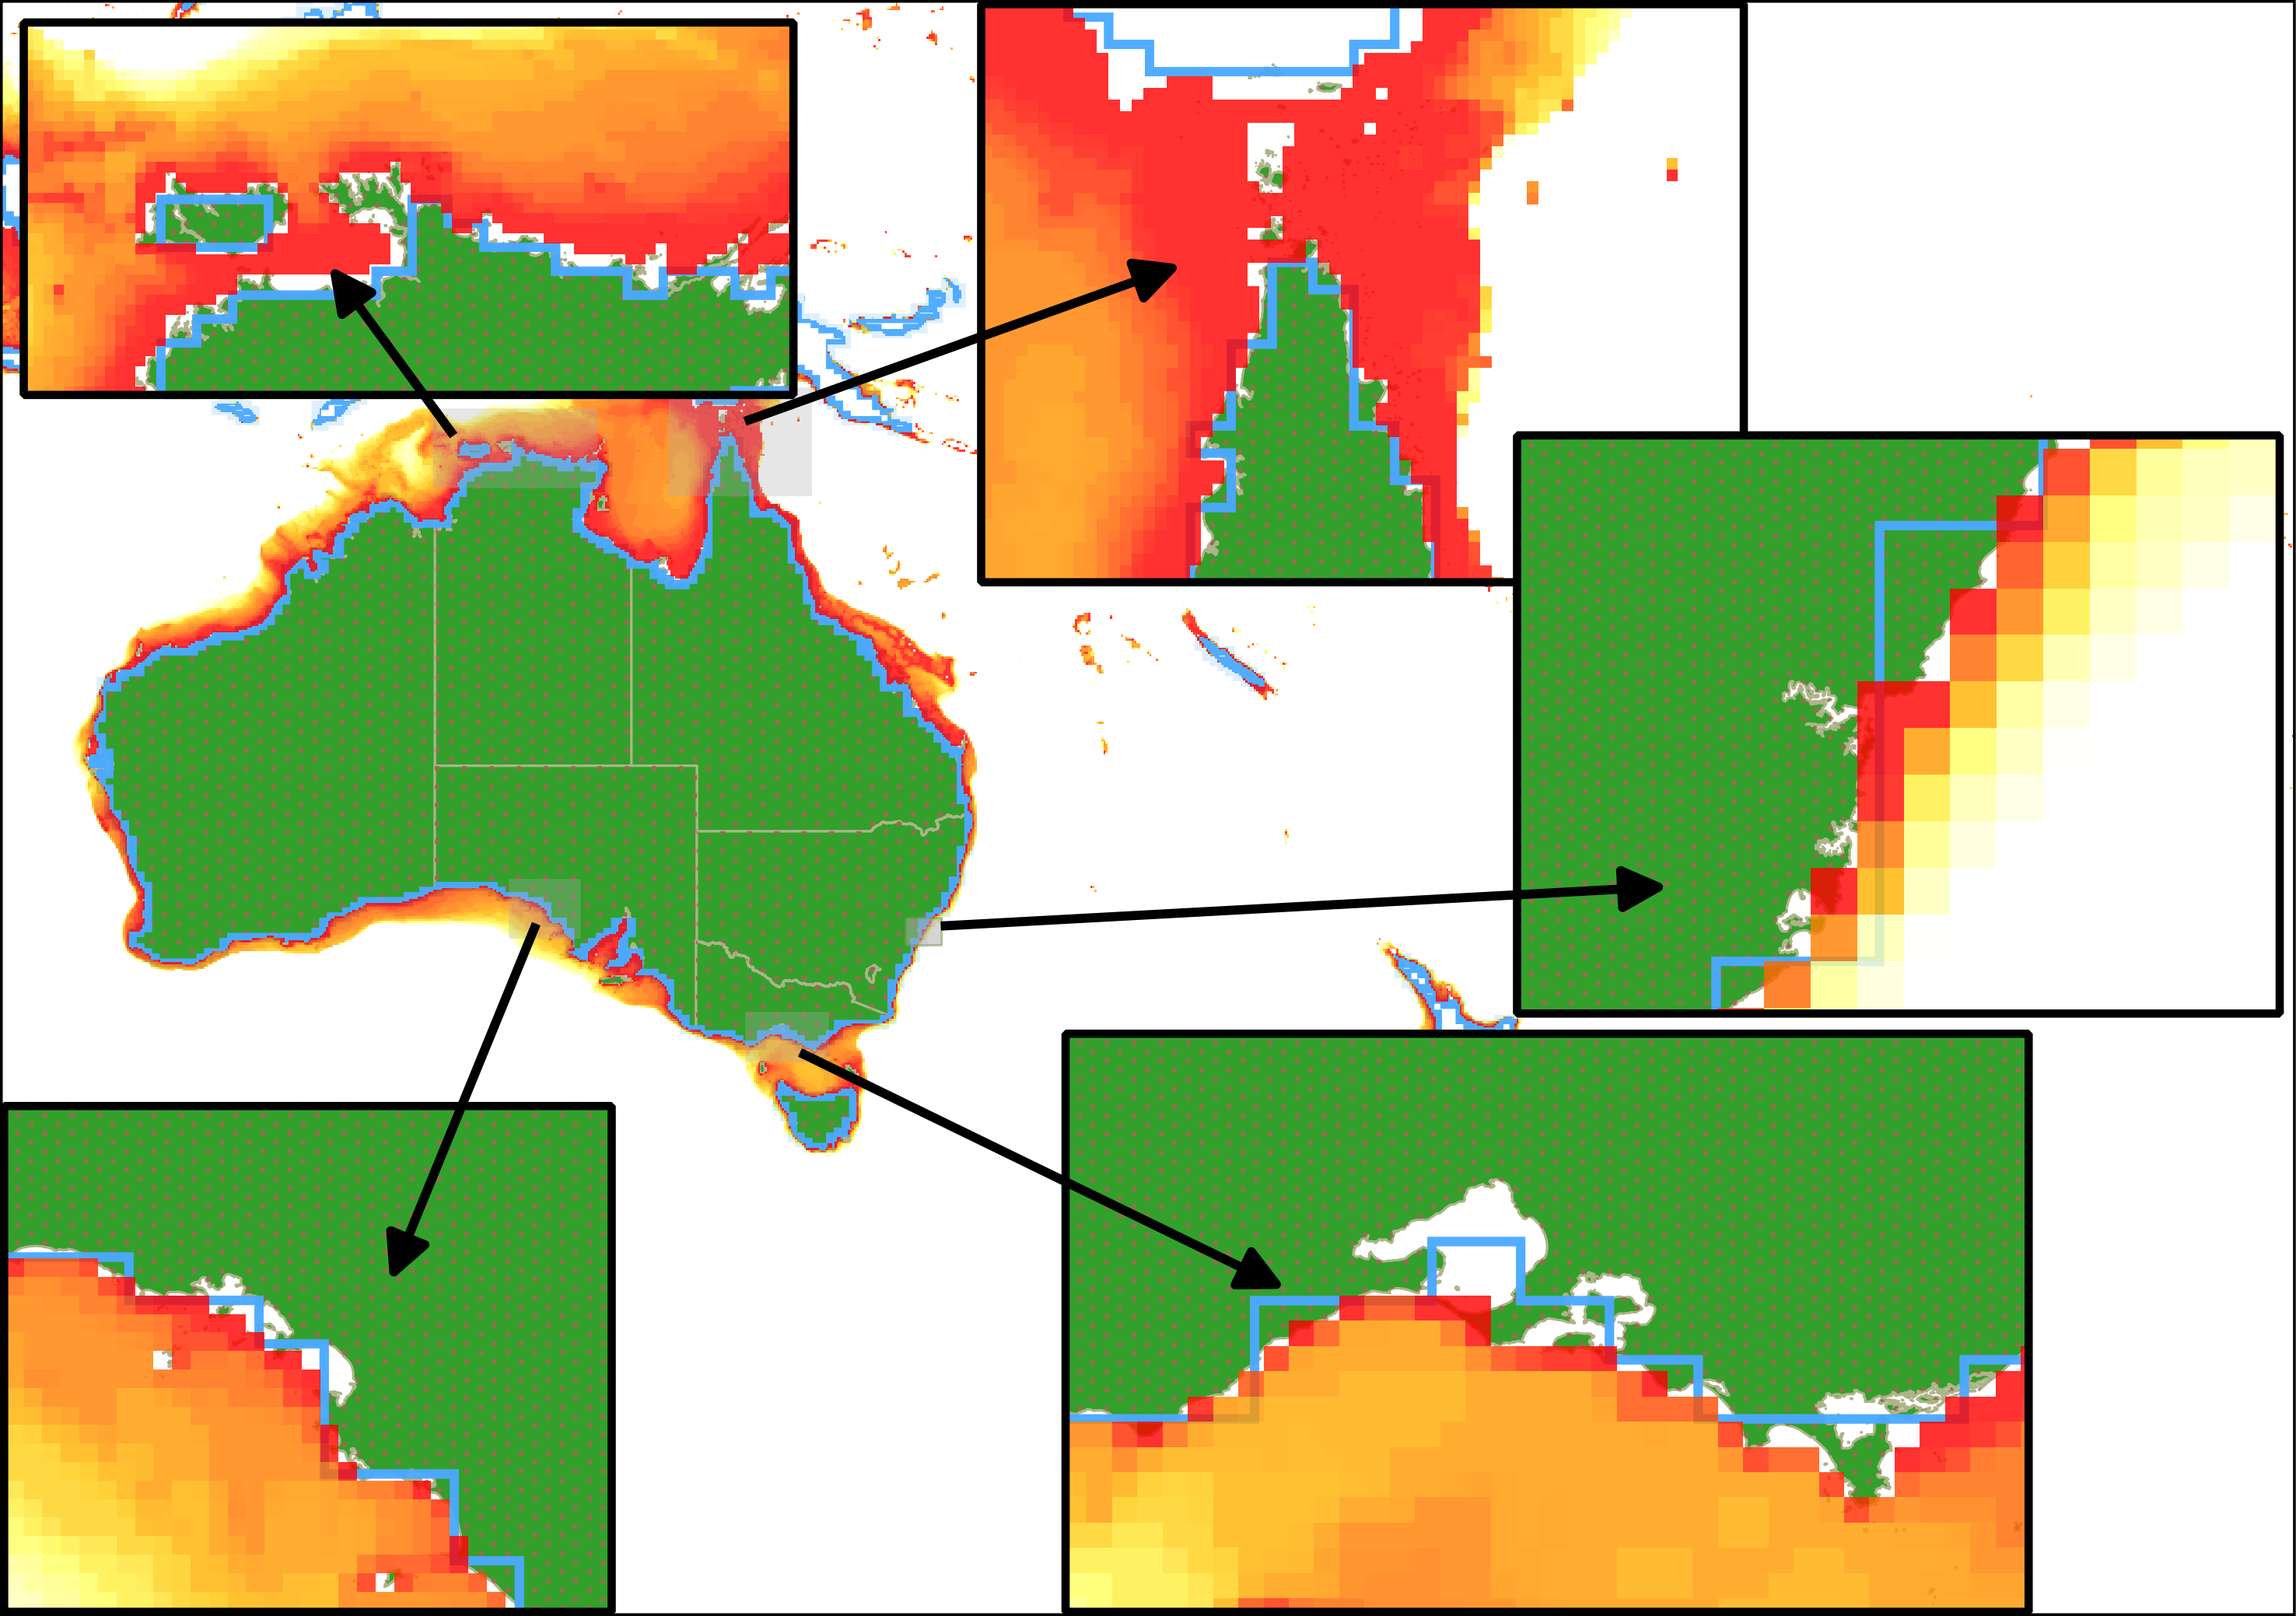
\includegraphics[width=\textwidth]{figures/maps/omaps_masks.png}
    \end{figure}
\end{frame}
%-----------------------------------------
\begin{frame}
\frametitle{characterise geographic distribution of skill}
\begin{columns}
    %--------------
    \begin{column}{0.3\textwidth}
      \begin{figure}      
        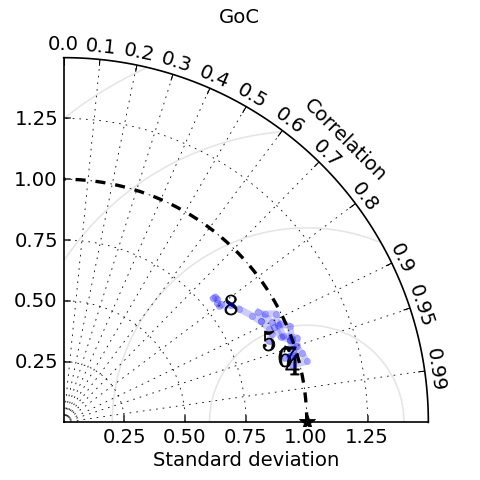
\includegraphics[width=\textwidth]{figures/plots/taylor_diag_res_GoC.png}
      \end{figure}
      \begin{figure}      
        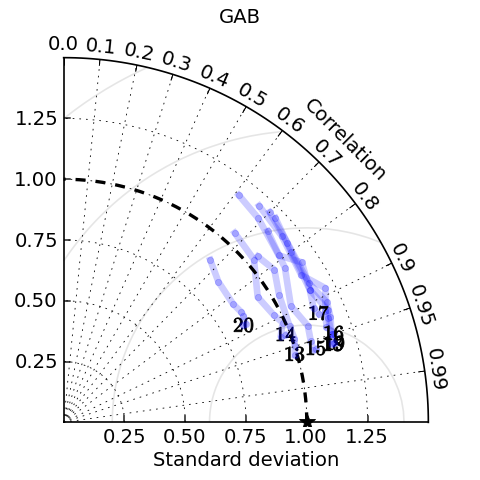
\includegraphics[width=\textwidth]{figures/plots/taylor_diag_res_GAB.png}
      \end{figure}
    \end{column}
    %--------------
    \begin{column}{0.3\textwidth}
      \begin{figure}      
        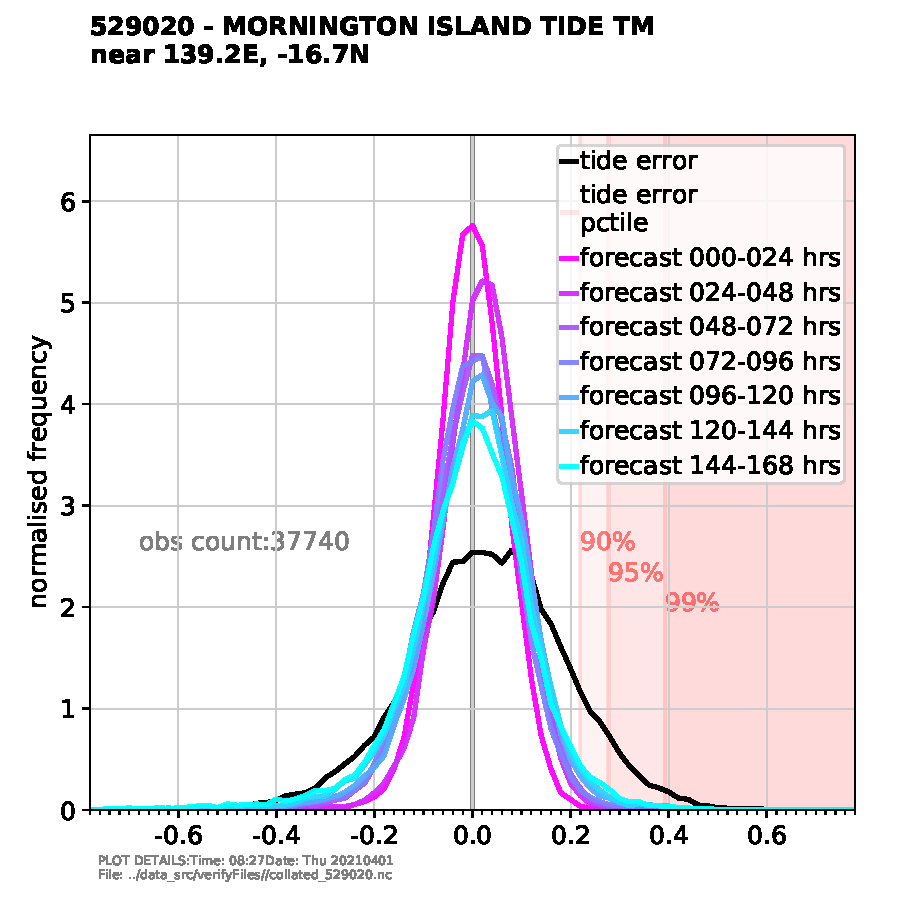
\includegraphics[width=\textwidth]{figures/plots/529020_plot_verify_pdf.pdf}
      \end{figure}
      \begin{figure}      
        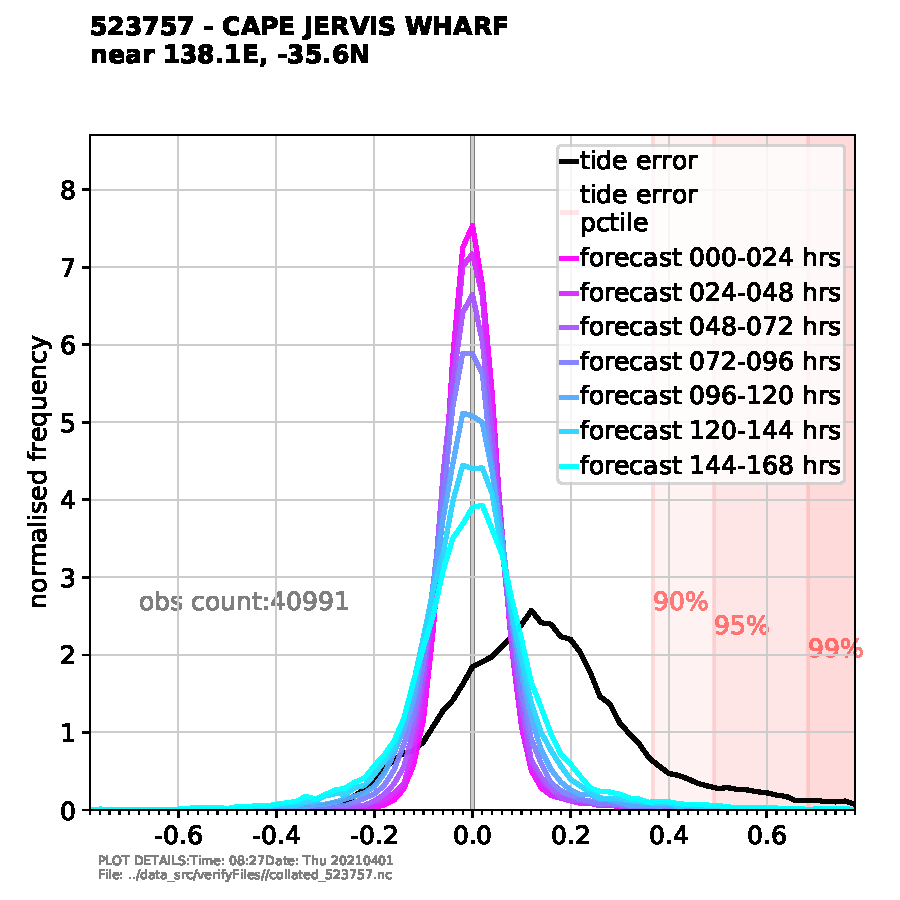
\includegraphics[width=\textwidth]{figures/plots/523757_plot_verify_pdf.pdf}
      \end{figure}
    \end{column}
    %--------------
    \begin{column}{0.3\textwidth}
      \begin{figure}      
        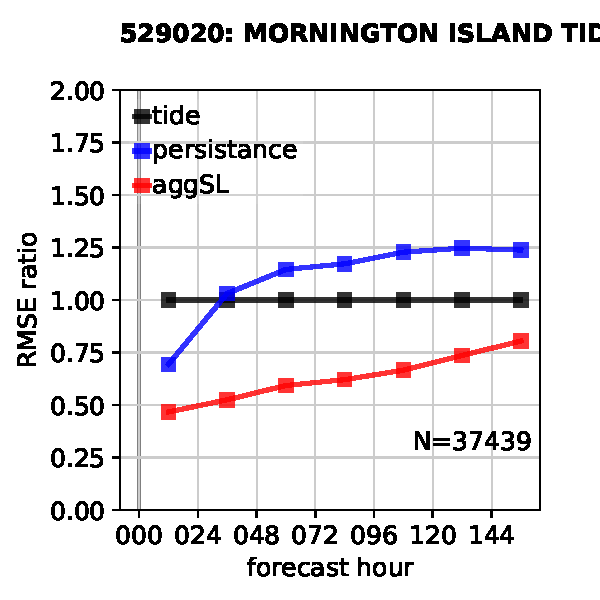
\includegraphics[width=\textwidth]{figures/plots/529020_verify_rms_growth.pdf}
      \end{figure}
      \begin{figure}      
        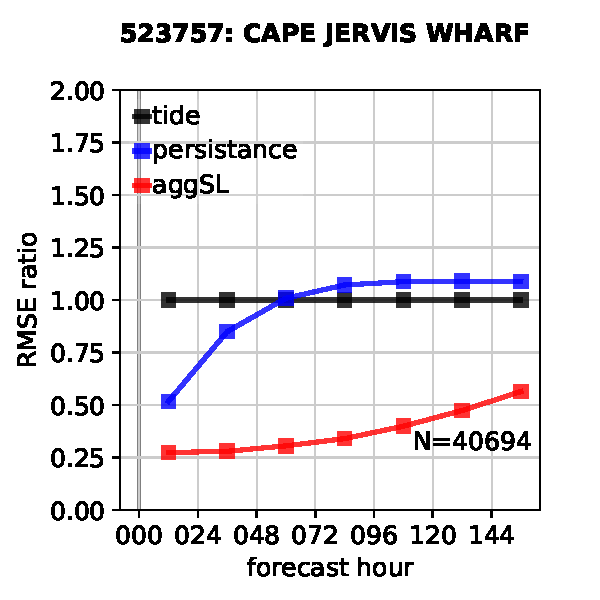
\includegraphics[width=\textwidth]{figures/plots/523757_verify_rms_growth.pdf}
      \end{figure}
    \end{column}
\end{columns}

\end{frame}

%-----------------------------------------
\begin{frame}
\frametitle{characterise geographic distribution of skill}

    %--------------
      \begin{figure}      
        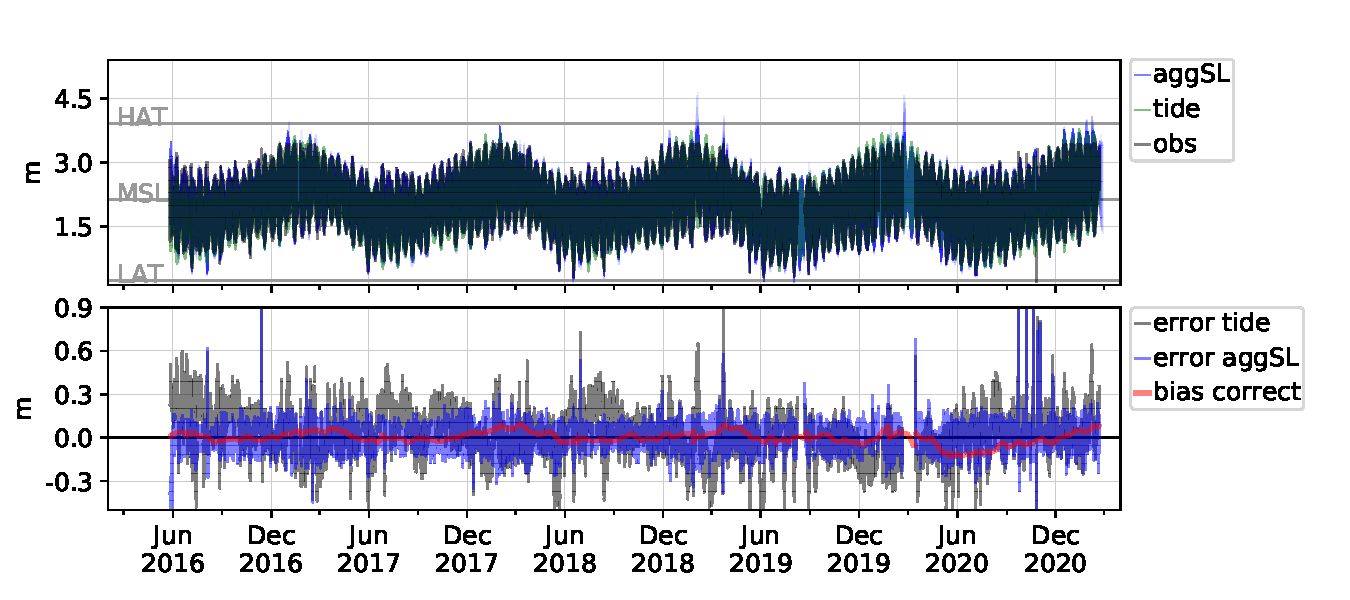
\includegraphics[height=0.4\textheight]{figures/plots/529020_verify_ts.pdf}
      \end{figure}
      \begin{figure}      
        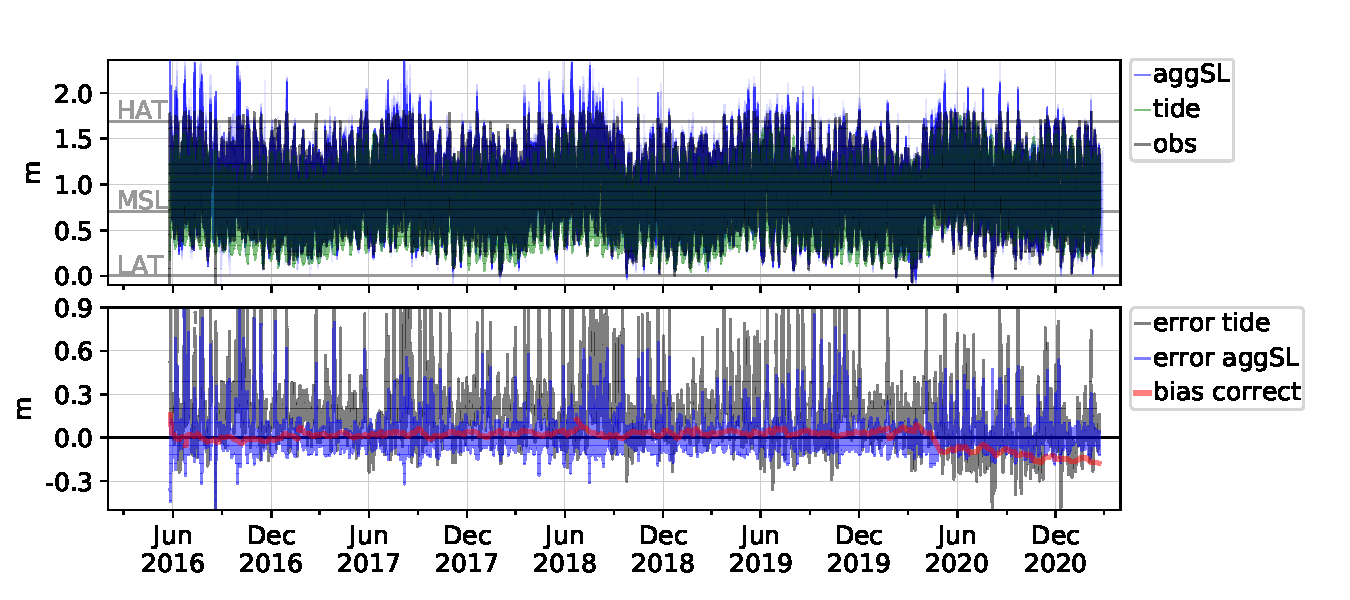
\includegraphics[height=0.4\textheight]{figures/plots/523757_verify_ts.pdf}
      \end{figure}

\end{frame}

%-----------------------------------------
\begin{frame}
\frametitle{interpretation of bias term}
\begin{columns}
    \begin{column}{0.4\textwidth}
      \begin{figure}      
        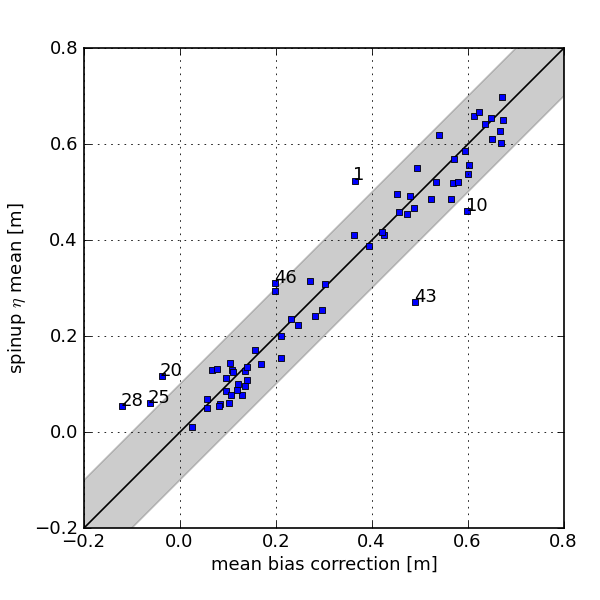
\includegraphics[width=\textwidth]{figures/plots/aggSL_bias_breakdown_plot_1.png}
      \end{figure}
    \end{column}

    \begin{column}{0.6\textwidth}
      \begin{figure}      
        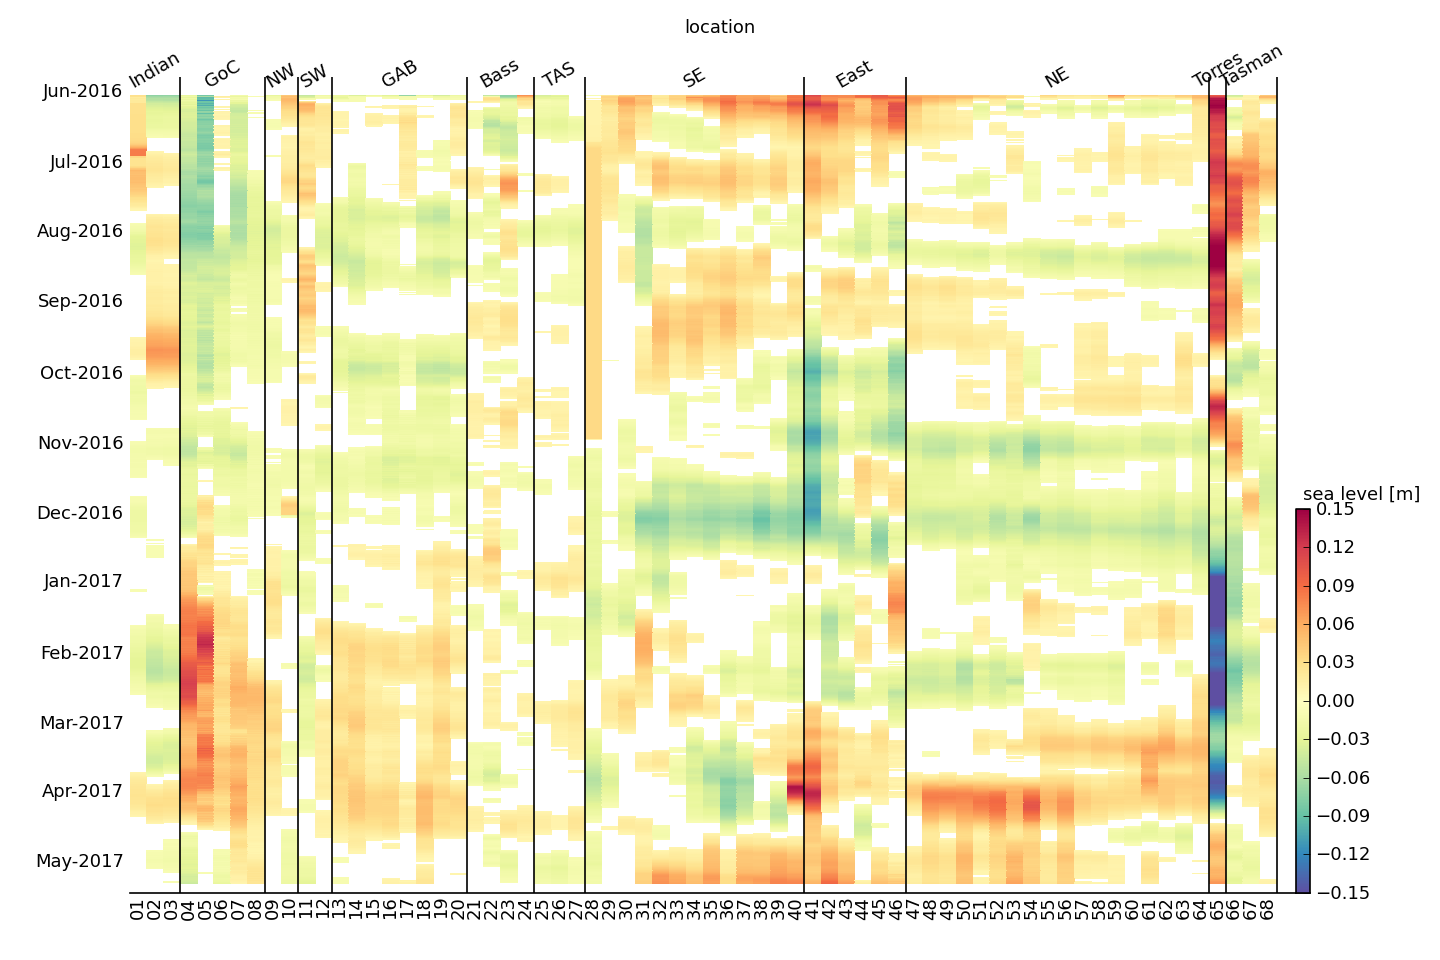
\includegraphics[width=\textwidth]{figures/plots/aggSL_bias_breakdown_plot_2.png}
      \end{figure}
    \end{column}
\end{columns}
\end{frame}
%-----------------------------------------
\begin{frame}
\frametitle{extrapolation along coast?}
\begin{columns}
    \begin{column}{0.5\textwidth}
      \begin{figure}      
        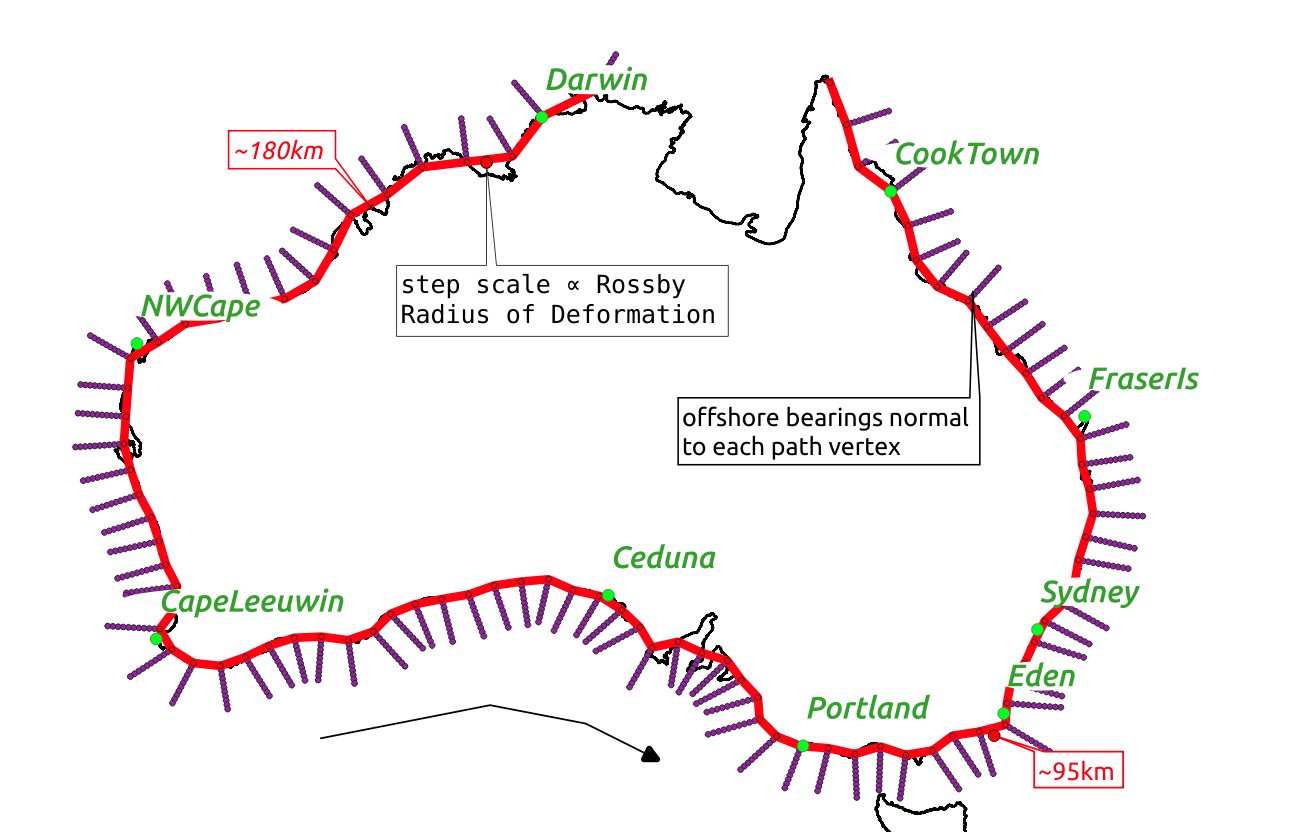
\includegraphics[width=\textwidth]{figures/maps/map_overview.png}
      \end{figure}
    \end{column}

    \begin{column}{0.5\textwidth}
      \begin{figure}      
        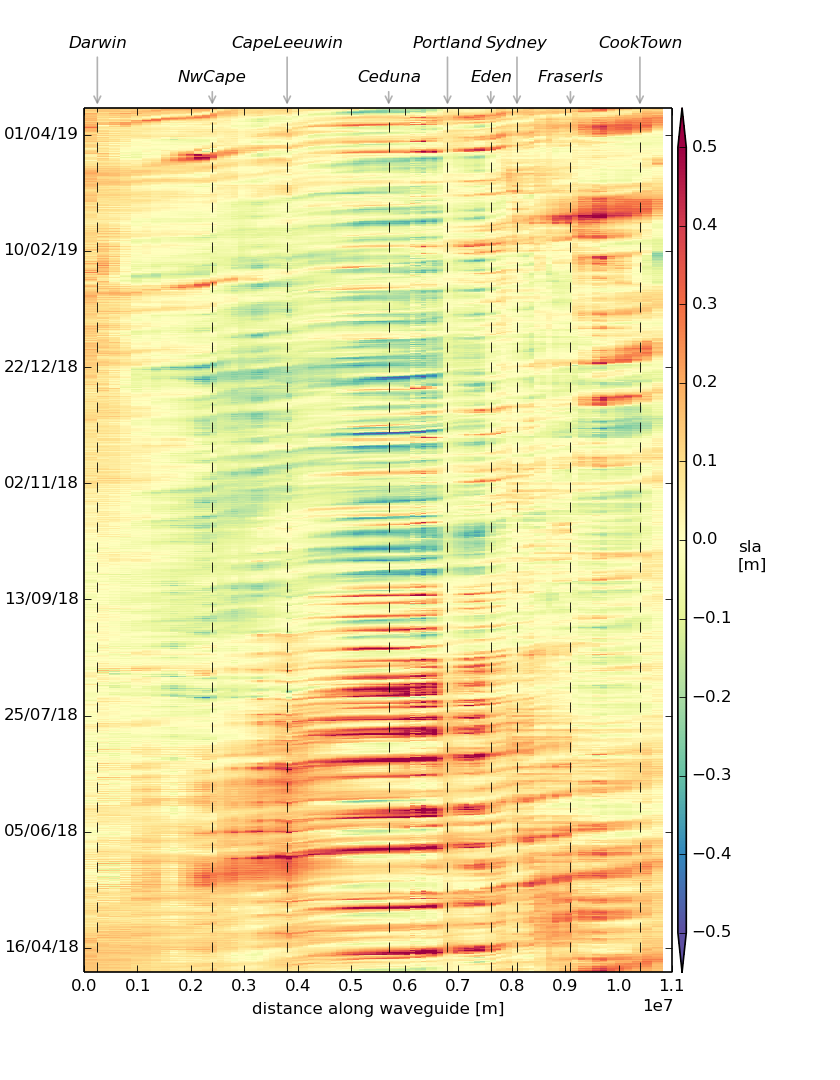
\includegraphics[width=\textwidth]{figures/plots/concat_sla_day0_full.png}
      \end{figure}
    \end{column}
\end{columns}
\end{frame}
%-----------------------------------------
\begin{frame}
\frametitle{double counting and adjustments}
\begin{columns}
    \begin{column}{0.5\textwidth}
      \begin{figure}      
        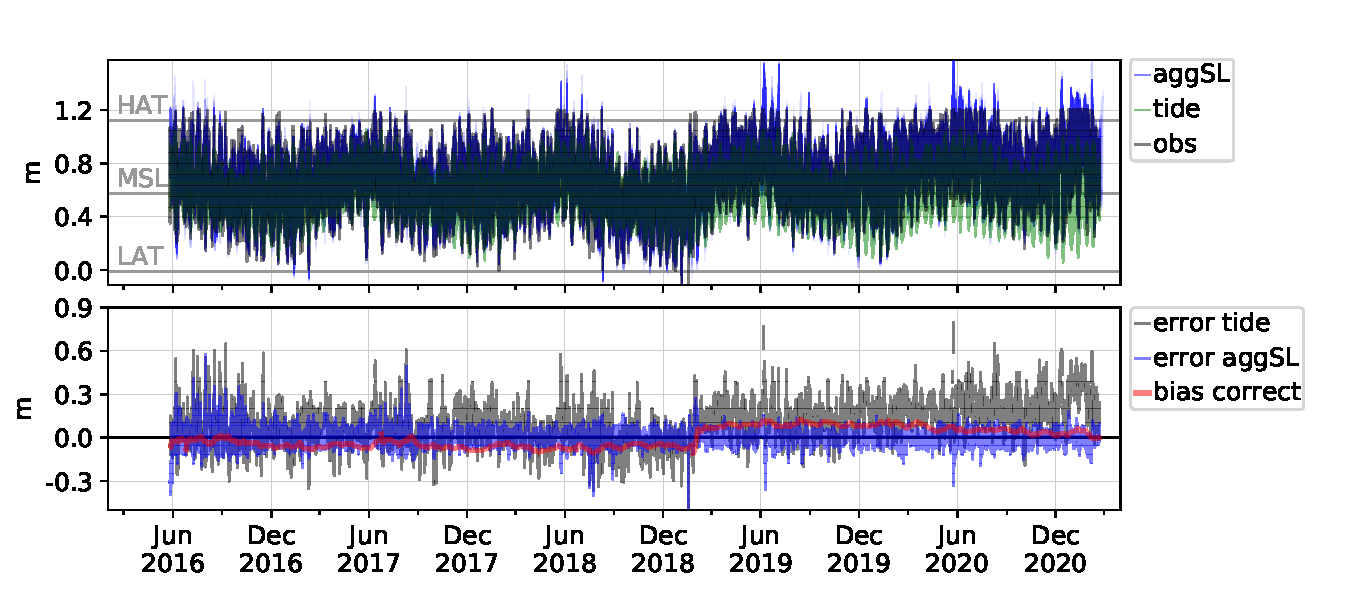
\includegraphics[width=\textwidth]{figures/plots/008314_verify_ts.pdf}
        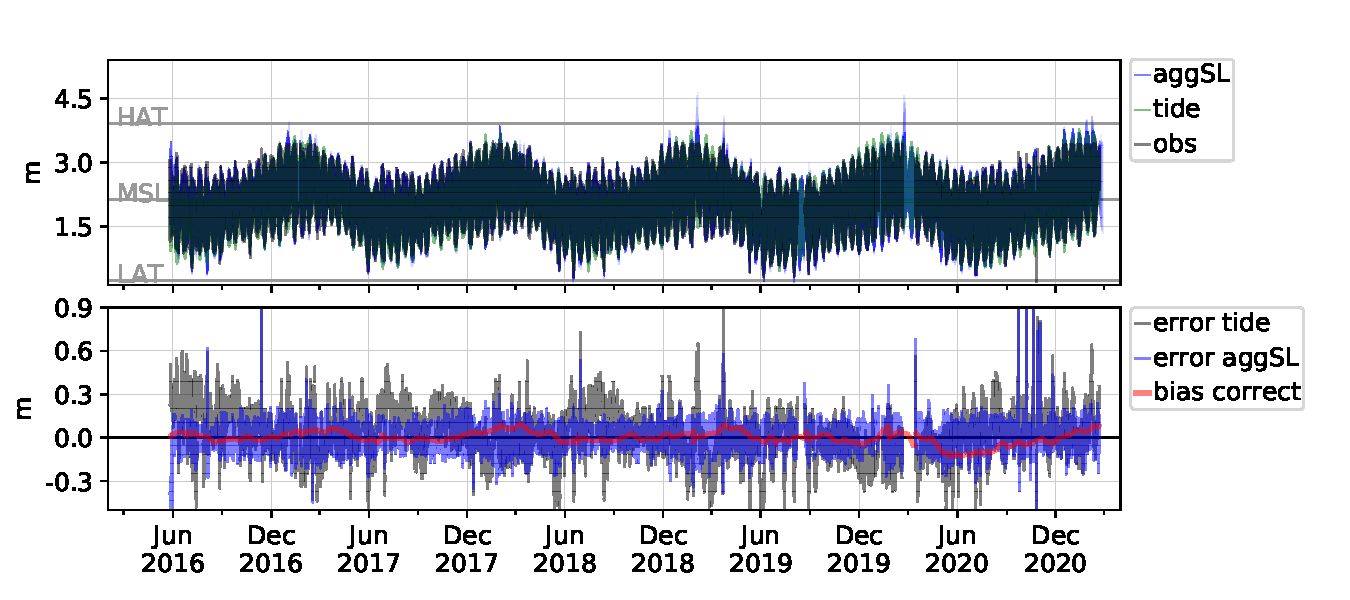
\includegraphics[width=\textwidth]{figures/plots/529020_verify_ts.pdf}
      \end{figure}
    \end{column}

    \begin{column}{0.5\textwidth}
      \begin{figure}      
        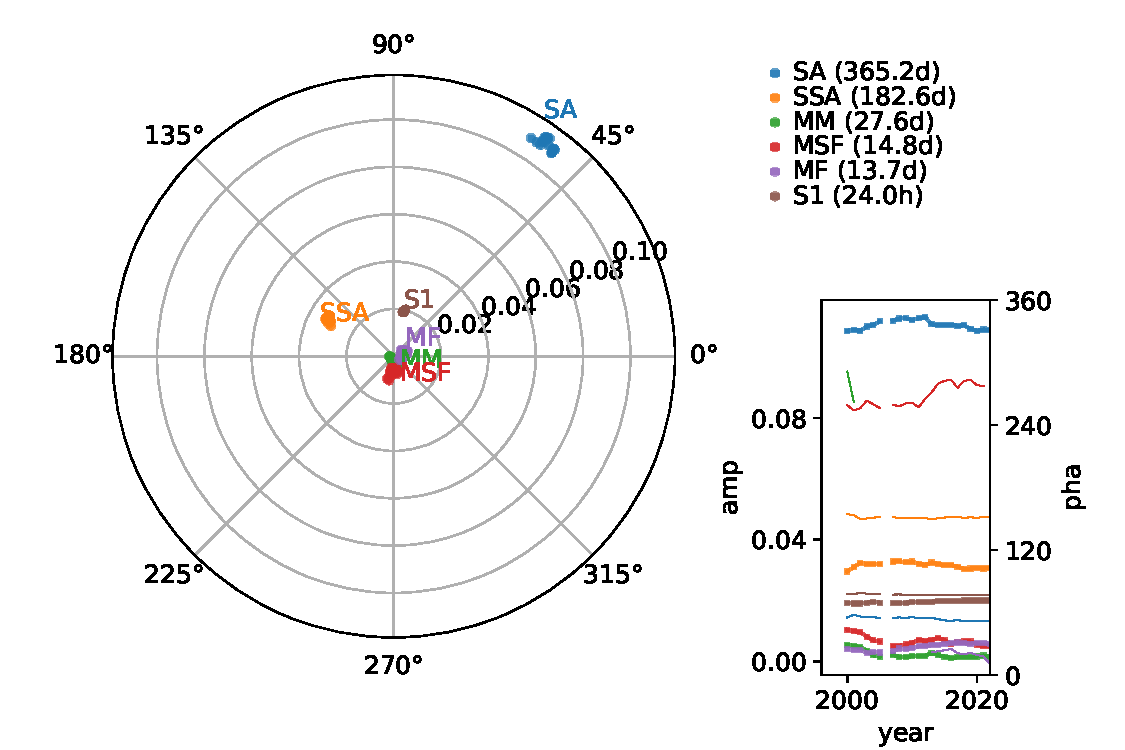
\includegraphics[height=0.4\textheight]{figures/plots/complex_62290.pdf}
        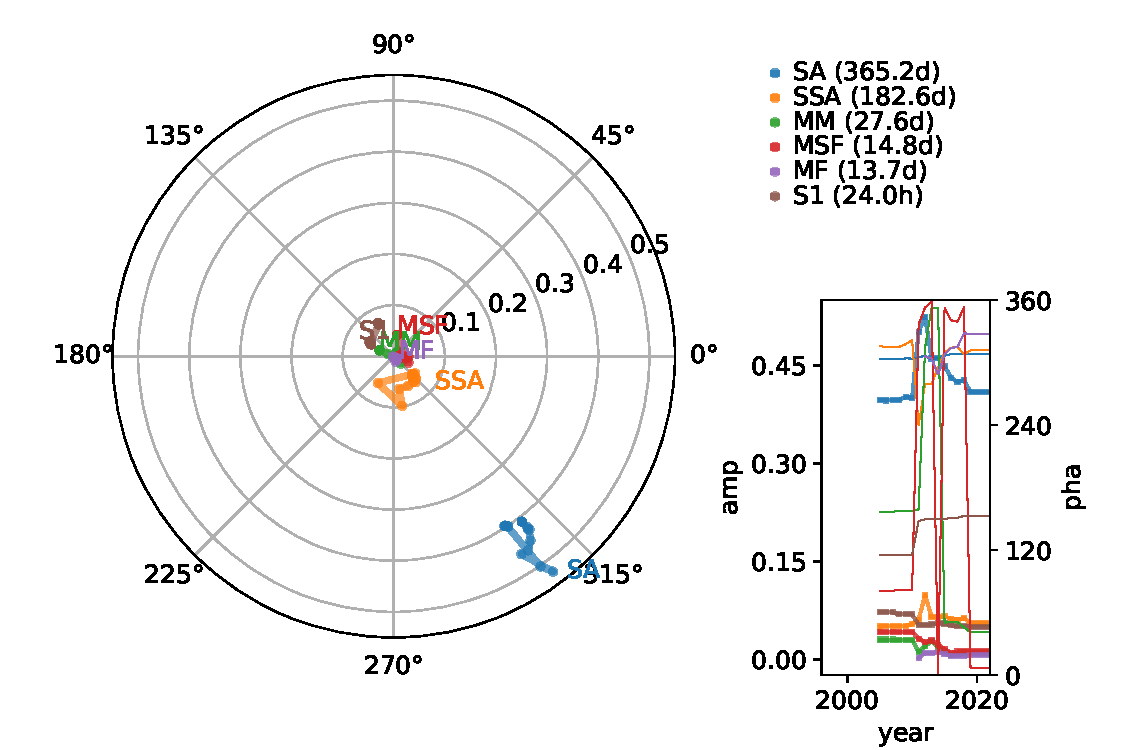
\includegraphics[height=0.4\textheight]{figures/plots/complex_63540.pdf}
      \end{figure}
    \end{column}
\end{columns}

\end{frame}
%-----------------------------------------
\begin{frame}
\frametitle{blunt adjustment - better ways to identify ``tide''}
\begin{itemize}
    \item old or academic innovations: response, orthotide, tidal wavelets
    \item essentially ignored for standard predictions
    \item lead into next section
\end{itemize} 
\end{frame}
%-----------------------------------------
%\begin{frame}
%\frametitle{tbc}
%\begin{minipage}{0.45\textwidth}
%    \begin{figure}      
%    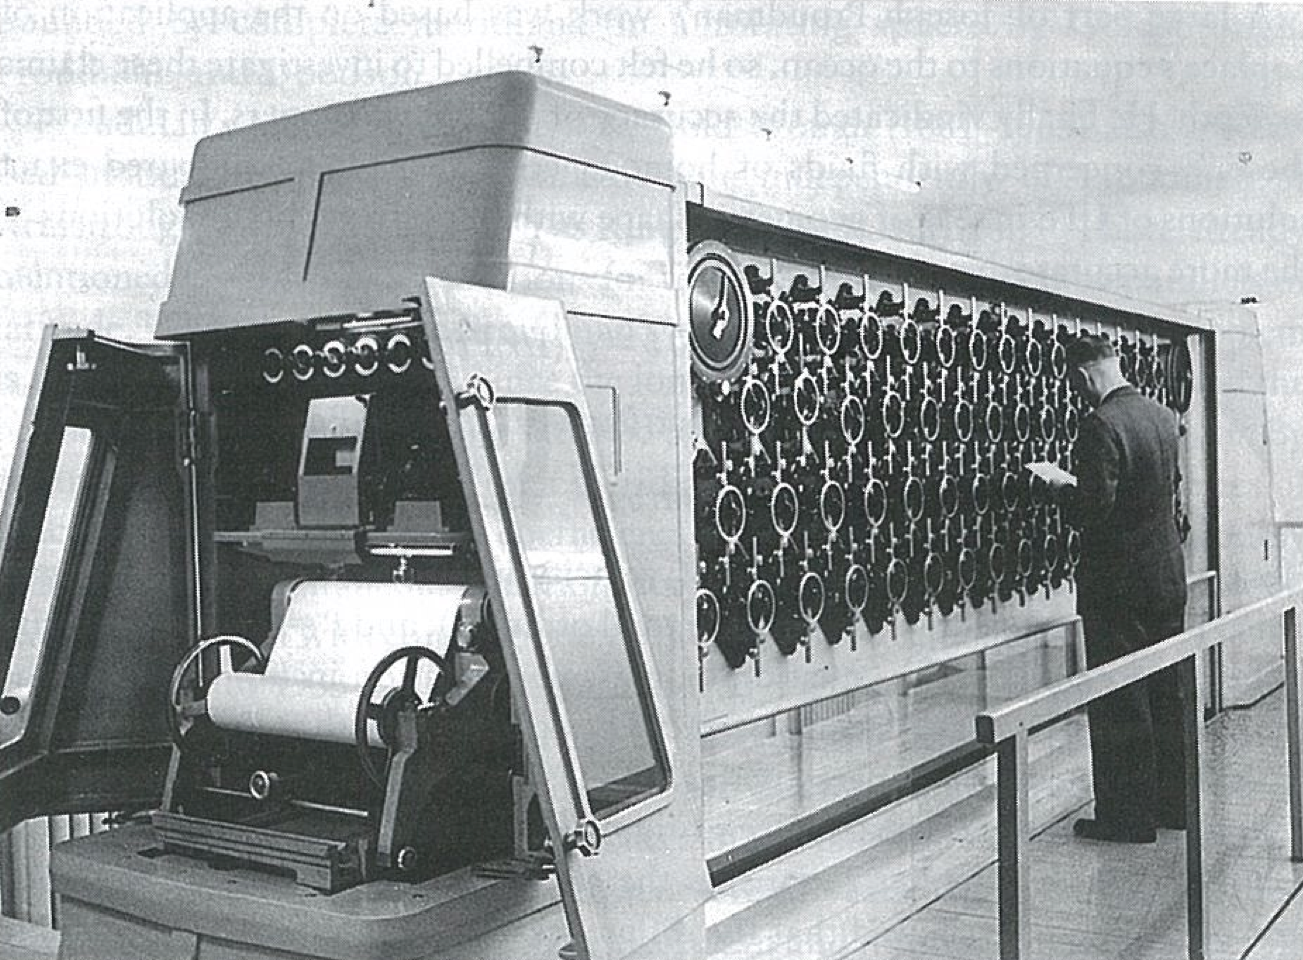
\includegraphics[width=\textwidth]{figures/images/DHI_machine_cartwright_fig11p2.png}
%    \end{figure}
%\end{minipage}
%\hfill
%\end{frame}